\documentclass[11pt,a4paper]{article}
\usepackage[utf8]{inputenc}
\usepackage[T1]{fontenc}
\usepackage[spanish,es-tabla]{babel}
\usepackage[margin=2cm]{geometry}
\usepackage{graphicx}
\usepackage[hidelinks]{hyperref}

\setlength{\parindent}{0pt}
\setlength{\parskip}{4pt}

\begin{document}

\noindent\begin{tabular}{@{}ll@{}}
\textbf{Apellidos y nombres:} & ROBINSON ESPINOZA JEANPIERRE\\
\textbf{Asignatura:} & Ingeniería de Requerimientos (ISR-401)\\
\textbf{Nivel y paralelo:} & 4.\textsuperscript{o} nivel, paralelo B\\
\textbf{Código y nombre de la tarea:} & EV-PRAC-01, Evaluación de la Unidad I\\
\textbf{Fecha de la sesión:} & 18 de noviembre de 2026\\
\textbf{Fecha límite de entrega:} & 18 de noviembre de 2026, 23:59\\
\textbf{URL del repositorio:} & \mbox{\url{https://github.com/jean200525/ISR-401-EV-PRAC-01-}}\\
\end{tabular}

\vspace{10pt}

\noindent\textbf{Resumen del cuestionario EV-CUE-01 resuelto en el SGA}

\vspace{6pt}

\noindent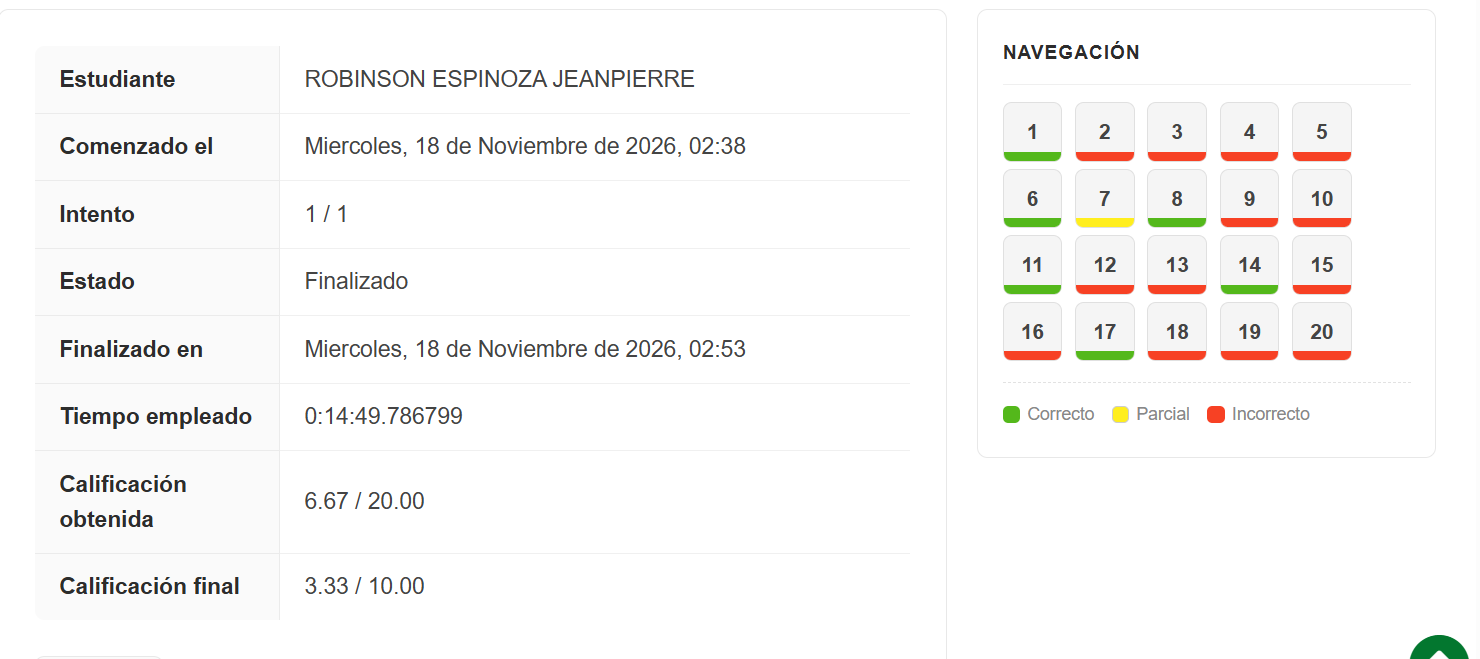
\includegraphics[width=\linewidth]{nota-ev.png}

\end{document}
